\label{sec:bosquejoGeneral}

\section{Arquitectura general}

	Con base en la teoría general de los sistemas según Ludwig von Bertalanffy, el sistema TLAMATINIME está conformado por tres sistemas. A continuación se detallan estos sistemas:
	
	\begin{itemize}
		\item \textbf{Sistema de Gestión de Información (SGI)}: Es el sistema encargado de gestionar la información requerida por el siguiente sistema.
		
		\item \textbf{Sistema Experto (SE)}: En este se encuentra el algoritmo que se ejecutará para crear los horarios correspondientes. Una vez que se obtienen las posibles soluciones, estas se verán en el siguiente sistema.
		
		\item \textbf{Sistema de Soporte a las Decisiones (DSS)}: Finalmente, este sistema muestra los resultados del algoritmo permitiendo al responsable tomar la decisión de utilizar esta opción de horario o generar una nueva.
	\end{itemize}
	
	En la figura~\ref{fig:sistemaT} se muestra la estructura de los sistemas que conforman al sistema en conjunto.

	\begin{figure}[htbp!]
		\begin{center}
			\fbox{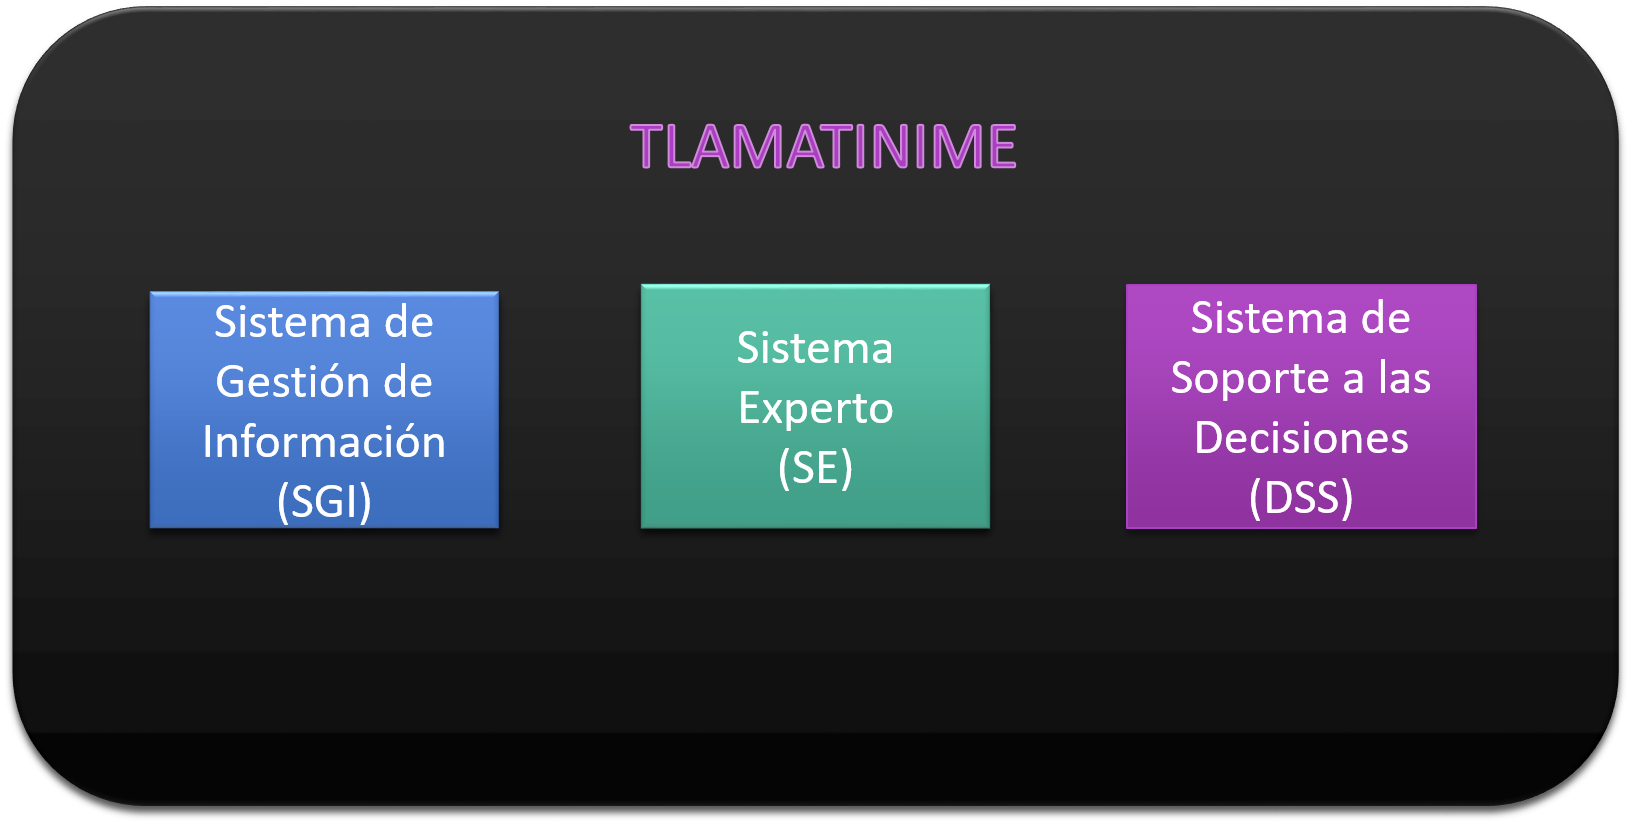
\includegraphics[width=.5\textwidth]{images/entornoTT/TLAMATINIME.png}}
			\caption{Modelo del sistema.}
			\label{fig:sistemaT}
		\end{center}
	\end{figure}

	

\section{Componentes}

	En la figura~\ref{fig:paquetes} se muestra el diagrama de paquetes que conforman al sistema.
	
	\begin{figure}[htbp!]
		\begin{center}
			\fbox{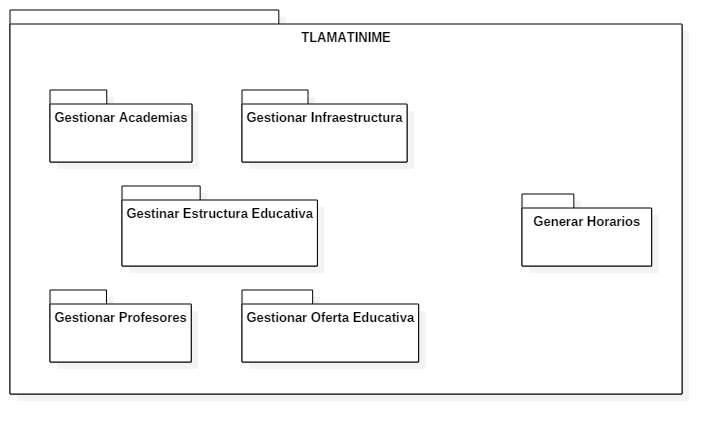
\includegraphics[width=.5\textwidth]{images/entornoTT/paquetes.png}}
			\caption{Diagrama de paquetes del sistemas.}
			\label{fig:paquetes}
		\end{center}
	\end{figure}
	

\section{Requerimientos}
	
	Los requerimientos de un sistema de software son frecuentemente clasificados como requerimientos funcionales y requerimientos no funcionales: 

\subsection{Requerimientos funcionales}
	Estos son sentencias de los servicios que el sistema debería proporcionar, como el sistema debería reaccionar para entradas particulares, y como el sistema debería comportarse en situaciones particulares. En algunos casos, los requerimientos funcionales pueden decir explícitamente lo que el sistema no debe hacer. \\
	
	A continuación se enlistan los requerimientos funcionales identificados para el sistema.	
	
	\begin{itemize}
		\item El sistema debe permitir al subdirector académico seleccionar las unidades de aprendizaje que se impartirán durante un semestre.
		
		\item El sistema debe permitir al subdirector académico asignar a un profesor las unidades de aprendizaje que impartirá durante el semestre.
		
		\item El sistema debe permitir al subdirector académico consultar los horarios una vez generados.
		
		\item El sistema debe permitir al subdirector académico seleccionar un horario.
		
		\item El sistema debe permitir al subdirector académico realizar modificaciones al horario seleccionado.
		
		\item Un profesor tiene un número finito de unidades de aprendizaje que debe impartir al semestre.
		
		\item Un profesor no puede estar en dos clases al mismo tiempo.
		Las unidades de aprendizaje así como los grupos deben estar divididas por nivel.
		
		\item Las unidades teórico-prácticas tienen un espacio para sus clases de práctica.
		
		\item Una unidad de aprendizaje no puede ser impartida más de una vez en el mismo grupo.
		
		\item Se debe priorizar que los profesores tengan la carga que deberían tener.
		
	\end{itemize}
	

\subsection{Requerimientos no funcionales}
	
	Estas son restricciones en los servicios o funciones que ofrece el sistema. Estos incluyen restricciones de tiempo, restricciones del proceso de desarrollo, y restricciones impuestas por estándares. Estos frecuentemente aplican a los sistemas como un todo, en vez de aplicar a características o servicios individuales del sistema. \\
	
	A continuación se enlistan los requerimientos no funcionales con los que cumplirá el sistema.

	\begin{itemize}
		\item Escalabilidad.
		
		\item Adaptabilidad.
		
		\item Legibilidad.
		
		\item Trazabilidad.
		
		\item Facilidad de uso.
		
		\item Documentación.
		
	\end{itemize}